\documentclass[12pt, a4paper]{article}

\usepackage[hmargin=2.5cm, vmargin=2cm]{geometry}
\usepackage{amsthm, amssymb, mathtools, yhmath, graphicx}
\usepackage{fontspec, type1cm, titlesec, titling, fancyhdr, tabularx}
\usepackage{caption}
\usepackage{color}
\usepackage{hhline}
\usepackage{unicode-math}
\usepackage{nicefrac}
\usepackage[abbreviations]{siunitx}
\usepackage{comment}
\usepackage{float}
\usepackage{subcaption}

\usepackage[CheckSingle, CJKmath]{xeCJK}
\usepackage{CJKulem}
\usepackage{enumitem}
\usepackage[usenames, dvipsnames]{xcolor}
\usepackage{colortbl}
\usepackage{circuitikz}
%\setCJKmainfont[BoldFont=cwTex Q Hei]{cwTex Q Ming}
%\setCJKsansfont[BoldFont=cwTex Q Hei]{cwTex Q Ming}
%\setCJKmonofont[BoldFont=cwTex Q Hei]{cwTex Q Ming}
\setCJKmainfont[BoldFont=cwTeX Q Hei]{cwTeX Q Ming}

\def\normalsize{\fontsize{12}{18}\selectfont}
\def\large{\fontsize{14}{21}\selectfont}
\def\Large{\fontsize{16}{24}\selectfont}
\def\LARGE{\fontsize{18}{27}\selectfont}
\def\Huge{\fontsize{20}{30}\selectfont}

\titleformat{\section}{\bf\Large}{\arabic{section}}{24pt}{}
\titleformat{\subsection}{\large}{\arabic{subsection}.}{12pt}{}
\titlespacing*{\subsection}{0pt}{0pt}{1.5ex}

\parindent=24pt

\DeclarePairedDelimiter{\abs}{\lvert}{\rvert}
\DeclarePairedDelimiter{\norm}{\lVert}{\rVert}
\DeclarePairedDelimiter{\inpd}{\langle}{\rangle}
\DeclarePairedDelimiter{\ceil}{\lceil}{\rceil}
\DeclarePairedDelimiter{\floor}{\lfloor}{\rfloor}

\newcommand{\unit}[1]{\:(\text{#1})}
\newcommand{\img}{\mathsf{i}}
\newcommand{\ex}{\mathsf{e}}
\newcommand{\dD}{\mathrm{d}}
\newcommand{\dI}{\,\mathrm{d}}
\DeclareSIUnit \uF {\micro \farad}
\DeclareSIUnit \mH {\milli \henry}

\title{ \bf {\huge 電子電路實驗8:運算放大器}\\ 實驗預報}
\author{B02901178 江誠敏}
%\date{2014/09/21}

\begin{document}

\maketitle

\section{實驗目的}
\begin{enumerate}[itemsep=0pt]
  \item 藉由運算放大器 IC 的操作了解 IC 封裝的基本規格。
  \item 了解基本的運算放大器電路。
  \item 對於運算放大器功能的驗證及應用。
\end{enumerate}


\section{實驗步驟}
將示波器之操作模式設於 X-Y mode。分別以矽二極體、鍺二極體、齊納二極體,以及$\SI{5.1}\kohm, \SI{100}\ohm$電阻,進行下列步驟:
\begin{enumerate}[itemsep=0pt]
  \item 按照μA741的接腳,將電路接成如圖 8.2(a) 的反相放大器,其中$R_1 = R_2 = \SI{100}\ohm$,並令$v_i = \SI{0}\V$(即將R1直接接地)。請確認電源打開之後,IC 各接腳的電位值為pin7 $\approx +\SI{15}\V$,pin4 $\approx -\SI{15}\V$,pin2, pin3, pin6$\approx \SI{0}\V$ 。如果全部正確,才繼續下一步驟。
  \item 令$v_i$為峰對峰值$\SI{100}\mV$的弦波($\SI{100}\mV$是信號產生器已接上電路的值),頻率依照每個數量級(decade)1, 2, 5 的順序由$\SI{20}\Hz$變化至$\SI{2}\MHz$,記錄$v_o$的峰對峰值。此值以橫軸為頻率,縱軸為$v_o / v_i$,以全對數紙將振幅畫出,可以描繪此反相放大器的波德圖(Bode Plot)。
  \item 將$R_2$ 改為$\SI{4.7}\kohm$,重複步驟2。
  \item 請按照 μA741 的接腳,將電路接成如圖 8.2(b) 的非反相放大器,其中$R_1 = R_2 = \SI{100}\ohm$,並令$v_i = \SI{0}\V$(即將$R_1$直接接地)。請確認電源打開之後,IC 各接腳的電位值為pin7 $\approx +\SI{15}\V$,pin4 $\approx -\SI{15}\V$,pin2, pin3, pin6$\approx \SI{0}\V$ 。如果全部正確,才繼續下一步驟。
  \item 令$v_i$為峰對峰值$\SI{100}\mV$的弦波($\SI{100}\mV$是信號產生器已接上電路的值),頻率依照每個數量級(decade)1, 2, 5 的順序由$\SI{20}\Hz$變化至$\SI{2}\MHz$,記錄$v_o$的峰對峰值。此值以橫軸為頻率,縱軸為$v_o / v_i$,以全對數紙將振幅畫出,可以描繪此非反相放大器的波德圖(Bode Plot)。
  \item 將$R_2$ 改為 $\SI{4.7}\kohm$,重複步驟 5。
  \item 請按照 μA741 的接腳,將電路接成如圖 8.3 的電壓隨耦器,並令$v_i = \SI{0}\V$ (即將$R_1$ 直接接地)。請確認電源打開之後,IC 各接腳的電位值為pin7 $\approx +\SI{15}\V$,pin4 $\approx -\SI{15}\V$,pin2, pin3, pin6$\approx \SI{0}\V$ 。如果全部正確,才繼續下一步驟。
  \item 令$v_i$為峰對峰值$\SI{100}\mV$的弦波($\SI{100}\mV$是信號產生器已接上電路的值),頻率依照每個數量級(decade)1, 2, 5 的順序由$\SI{20}\Hz$變化至$\SI{2}\MHz$,記錄$v_o$的峰對峰值。此值以橫軸為頻率,縱軸為$v_o / v_i$,以全對數紙將振幅畫出,可以描繪此電壓隨耦器的波德圖。
\end{enumerate}


\section{預報問題}

\begin{enumerate}[itemsep=20pt, topsep=10pt]
  \item {\large\bf μA741的各個接腳的用途為何?} \\[10pt]
    跟據μA741的datasheet\footnote{http://www.ti.com/lit/ds/symlink/ua741.pdf},可知
    \begin{figure}[H]
      \centering
      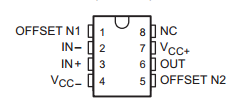
\includegraphics[width=6cm]{img/p1.png}
    \end{figure}
    \begin{enumerate}[label=pin \arabic*:, labelindent=0cm, leftmargin=*]
      \item Offset N1,與Offset N2合用來校正誤差,當兩個input端short時output電壓理論上應為0,但在實際上受許多因素影響導致偏差,因此可將此兩端以可變電阻連接修正。
      \item IN$-$,Inverting Input.
      \item IN$+$,Noninverting Input.
      \item VCC$-$,負電源供應。
      \item Offset N2,同Offset N1。
      \item OUT,輸出電壓端。
      \item VCC$+$,正電源供應。
      \item NC,Not connected,沒有功能。
    \end{enumerate}
    \clearpage
  \item {\large\bf 請用 PSpice 或其他電路模擬軟體模擬圖 8.2 與圖 8.3 的三個電路,其中 R1 與 R2 請比照實
驗步驟的設定。} 
  \begin{figure}[H]
    \centering
    \begin{subfigure}[b]{0.45\textwidth}
      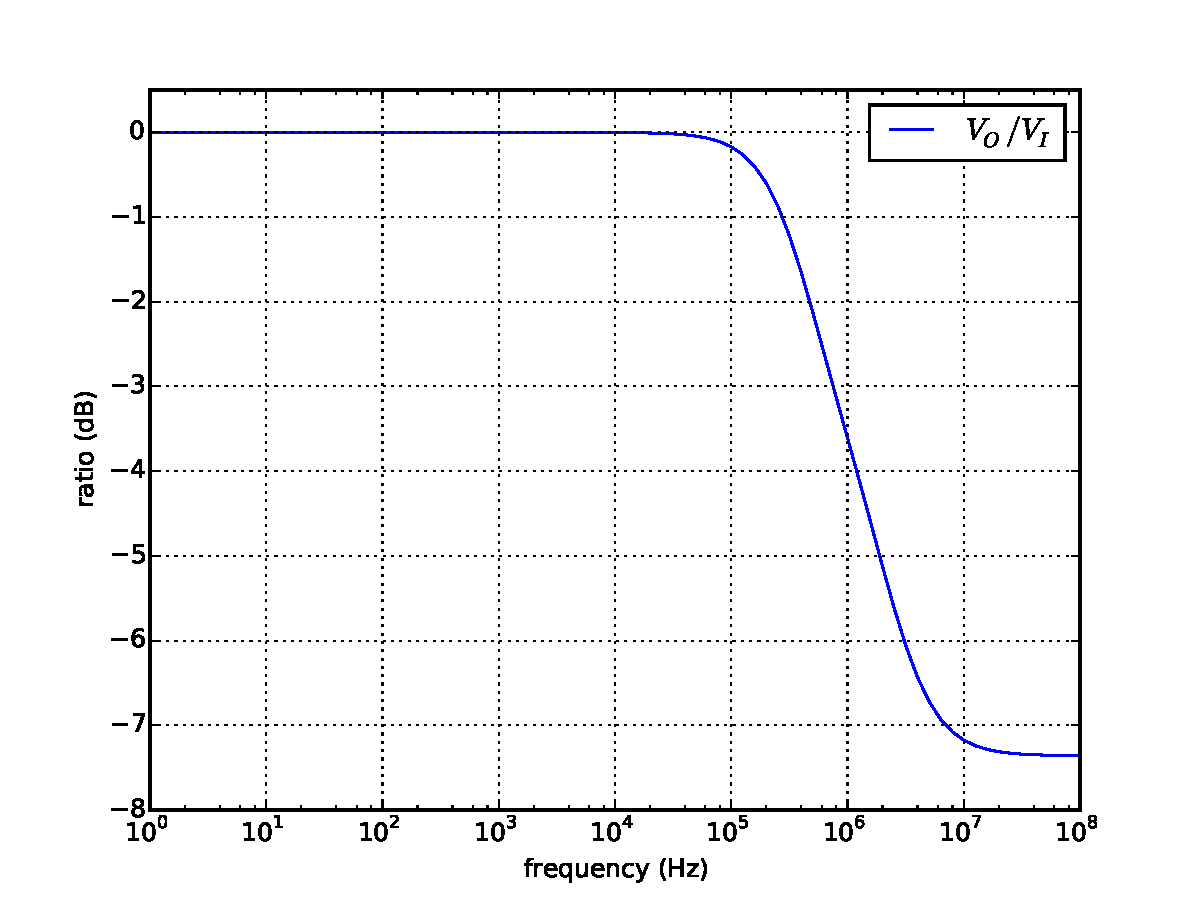
\includegraphics[width=1\textwidth]{circuit/p1.pdf}
      \caption{$\SI{100}\ohm$}
    \end{subfigure}
    \begin{subfigure}[b]{0.45\textwidth}
      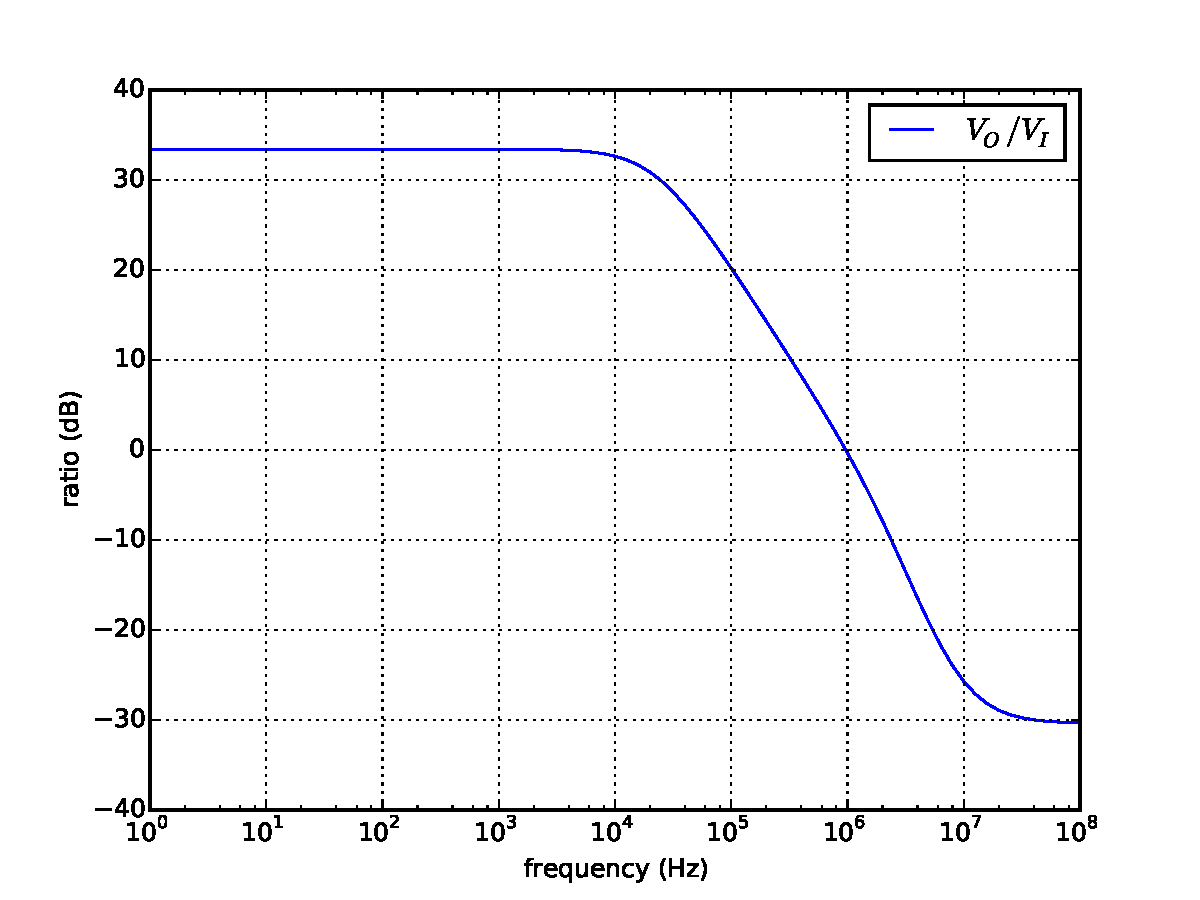
\includegraphics[width=1\textwidth]{circuit/p2.pdf}
      \caption{$\SI{4.7}\kohm$}
    \end{subfigure}
    \caption{Inverting configuration}
  \end{figure}
  \begin{figure}[H]
    \centering
    \begin{subfigure}[b]{0.45\textwidth}
      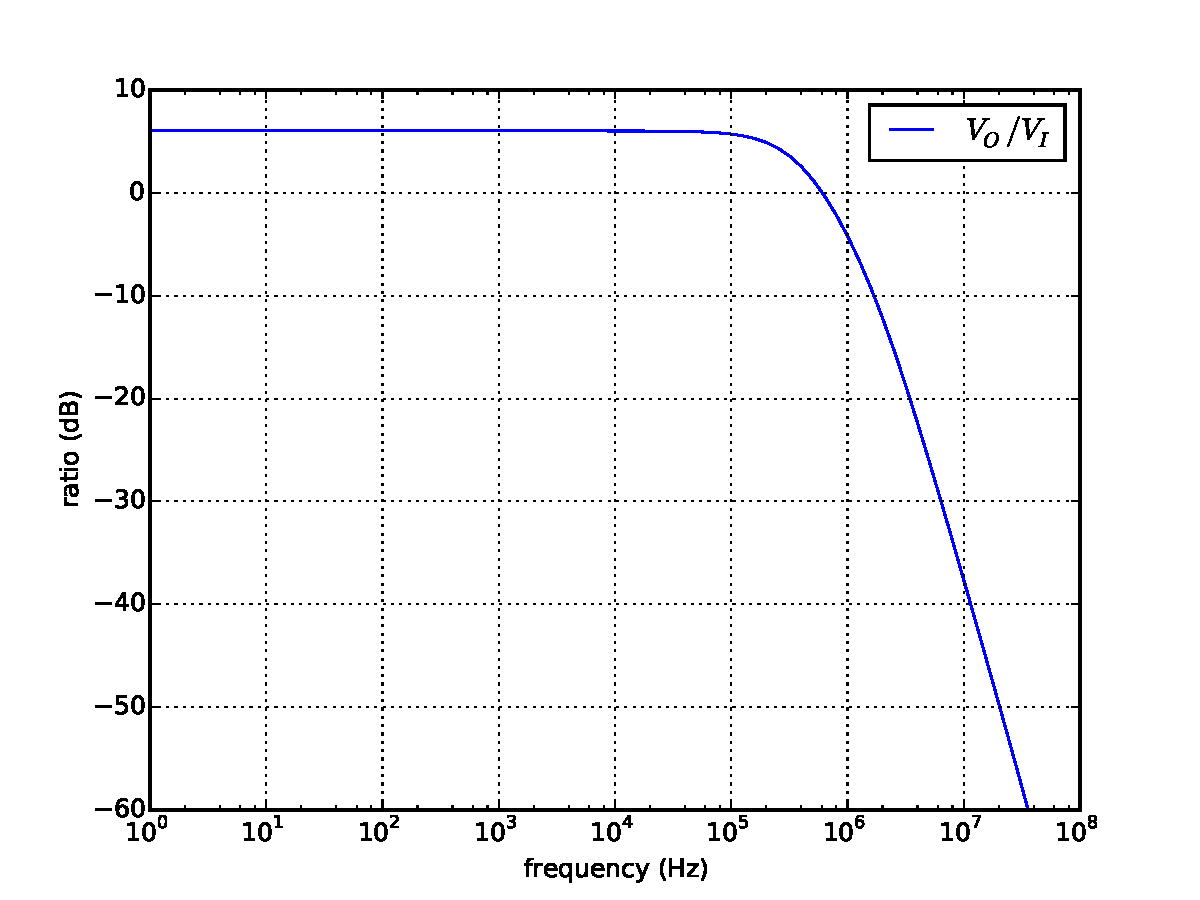
\includegraphics[width=1\textwidth]{circuit/p3.pdf}
      \caption{$\SI{100}\ohm$}
    \end{subfigure}
    \begin{subfigure}[b]{0.45\textwidth}
      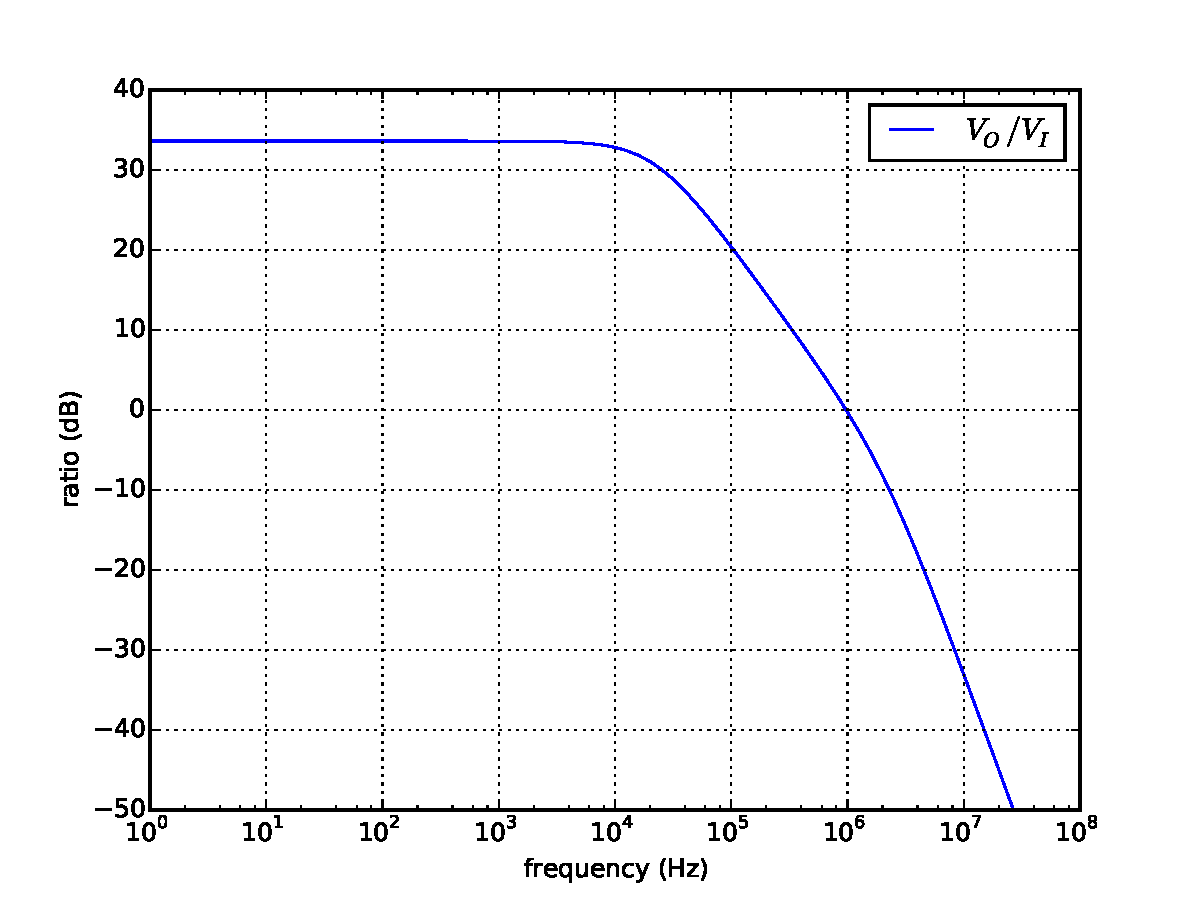
\includegraphics[width=1\textwidth]{circuit/p4.pdf}
      \caption{$\SI{4.7}\kohm$}
    \end{subfigure}
    \caption{Noninverting configuration}
  \end{figure}
  \begin{figure}[H]
    \centering
    \begin{subfigure}[b]{0.45\textwidth}
      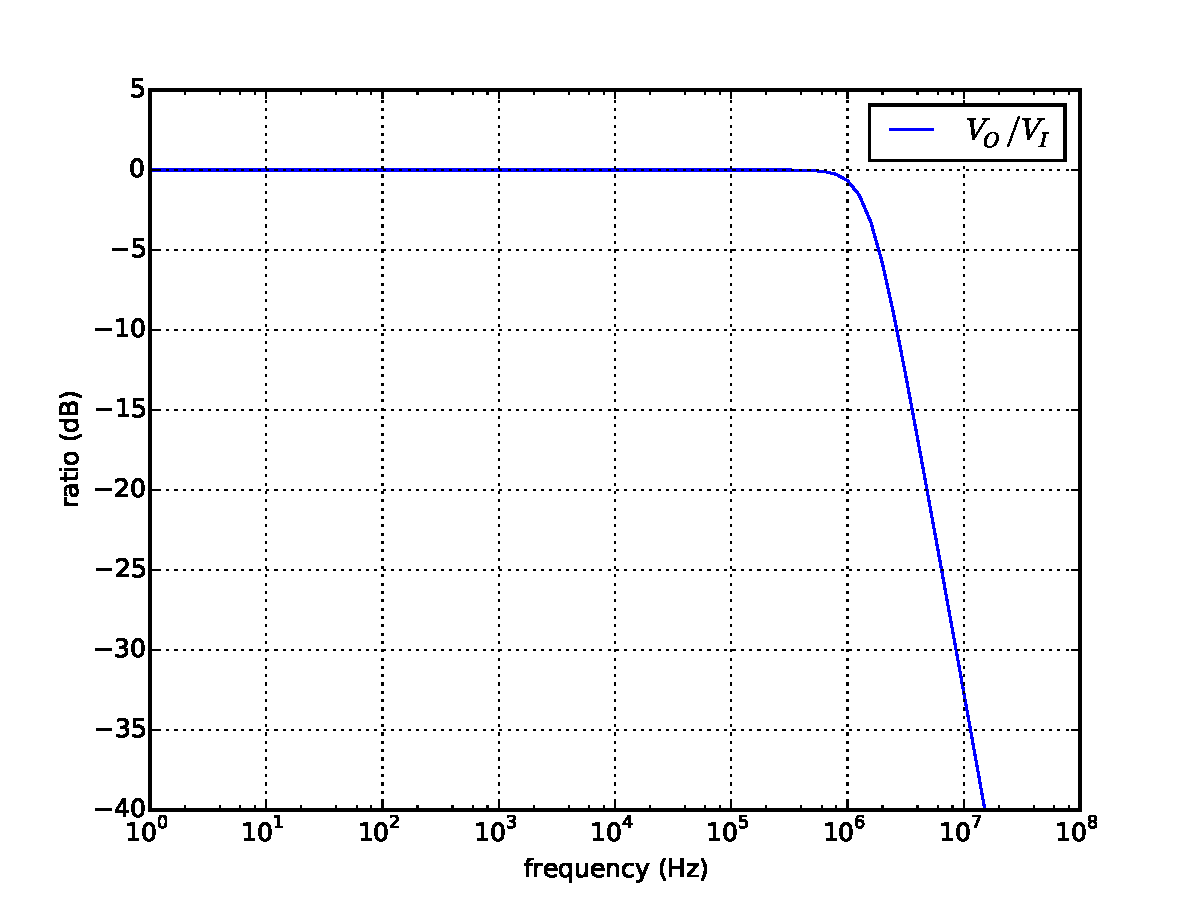
\includegraphics[width=1\textwidth]{circuit/p5.pdf}
    \end{subfigure}
    \caption{voltage follower}
  \end{figure}

\end{enumerate}

\end{document}


